\documentclass[a4paper,12pt]{article}

\usepackage[T2A]{fontenc}        
\usepackage[utf8]{inputenc}  
\usepackage[russian]{babel}

\usepackage[left=25mm, right=15mm, top=20mm, bottom=20mm]{geometry}


\usepackage{graphicx}
\usepackage{amsmath}
\usepackage{amssymb}
\usepackage{fancyhdr}
\usepackage{multirow}
\usepackage{cite}
\usepackage{hyperref}

\pagestyle{fancy}
\fancyhf{}
\fancyhead[L]{Домашнее задание }
\fancyhead[R]{Самир}
\fancyfoot[C]{\thepage}


\begin{document}
На рисунке~\ref{fig:zorich} представлен В.А. Зорич, автор упомянутого учебника~\cite{zorich}.
\tableofcontents
\newpage

\section{Математические формулы}

\subsection{Предел функции}

\setcounter{equation}{0}
\begin{equation}
\lim_{x\to0} \frac{\sin x}{x}=1
\label{eq:sin_limit}  
\end{equation}

\begin{equation}
\lim_{x\to0} (1+x)^\frac{1}{x}=e   
\end{equation}

\begin{equation}
\sum_{k=0}^{n} a_kD(D-1)...(D-k+1)y=0 
\end{equation}

\subsection{Производные}
Сводная информация по дифференцированию представлена в таблице~\ref{tab:derivatives}.
\setcounter{equation}{0}
\begin{equation}
\frac{d}{dx}(x^n) = nx^{n-1}
\end{equation}

\begin{equation}
\frac{d}{dx}(\sin x) = \cos x
\end{equation}

\begin{equation}
\frac{d}{dx}(\cos x) = -\sin x
\end{equation}

\begin{equation}
\frac{d}{dx}(e^x) = e^x
\end{equation}

\subsection{Интегралы}
\setcounter{equation}{0}

\begin{equation}
\int x^n dx = \frac{x^{n+1}}{n+1} + C
\end{equation}

\begin{equation}
\int \sin x dx = -\cos x + C
\end{equation}

\begin{equation}
\int \cos x dx = \sin x + C
\end{equation}

\begin{equation}
\int \frac{1}{x} dx = \ln|x| + C
\end{equation}

\subsection{Пределы и непрерывность}
\setcounter{equation}{0}

\begin{equation}
\lim_{x \to a} f(x) = L
\end{equation}

\begin{equation}
\lim_{x \to \infty} \frac{1}{x} = 0
\end{equation}

\begin{equation}
\lim_{x \to 0} \frac{1 - \cos x}{x^2} = \frac{1}{2}
\end{equation}

\begin{equation}
\lim_{x \to 0} \frac{\tan x}{x} = 1
\end{equation}

\begin{equation}
\lim_{x \to 0} \frac{e^x - 1}{x} = 1
\end{equation}

\subsection{Ряды}
\setcounter{equation}{0}

\begin{equation}
\sum_{n=1}^{\infty} \frac{1}{n^2} = \frac{\pi^2}{6}
\end{equation}

\begin{equation}
\sum_{n=0}^{\infty} x^n = \frac{1}{1-x}, \quad |x|<1
\end{equation}

\begin{equation}
e^x = \sum_{n=0}^{\infty} \frac{x^n}{n!}
\end{equation}

\begin{equation}
\sin x = \sum_{n=0}^{\infty} (-1)^n \frac{x^{2n+1}}{(2n+1)!}
\end{equation}

\begin{equation}
\cos x = \sum_{n=0}^{\infty} (-1)^n \frac{x^{2n}}{(2n)!}
\end{equation}

\subsection{Производные сложных функций}
\setcounter{equation}{0}

\begin{equation}
\frac{d}{dx}(f(g(x))) = f'(g(x)) \cdot g'(x)
\end{equation}

\begin{equation}
\frac{d}{dx}(\ln x) = \frac{1}{x}
\end{equation}

\begin{equation}
\frac{d}{dx}(\tan x) = \frac{1}{\cos^2 x}
\end{equation}

\begin{equation}
\frac{d}{dx}(\arcsin x) = \frac{1}{\sqrt{1-x^2}}
\end{equation}

\begin{equation}
\frac{d}{dx}(\arctan x) = \frac{1}{1+x^2}
\end{equation}

\subsection{Интегралы (расширенные)}
\setcounter{equation}{0}

\begin{equation}
\int e^x dx = e^x + C
\end{equation}

\begin{equation}
\int \frac{dx}{1+x^2} = \arctan x + C
\end{equation}

\begin{equation}
\int \frac{dx}{\sqrt{1-x^2}} = \arcsin x + C
\end{equation}

\begin{equation}
\int x e^x dx = (x-1)e^x + C
\end{equation}

\begin{equation}
\int \ln x  dx = x \ln x - x + C
\end{equation}

\subsection{Формула Тейлора (одна переменная)}
\setcounter{equation}{0}

\begin{equation}
f(x) = f(a) + f'(a)(x-a) + \frac{f''(a)}{2!}(x-a)^2 + \dots + \frac{f^{(n)}(a)}{n!}(x-a)^n + R_n
\end{equation}

Остаточный член:
\begin{equation}
R_n = \frac{f^{(n+1)}(\xi)}{(n+1)!}(x-a)^{n+1}
\end{equation}

\subsection{Дифференциальное исчисление}
\setcounter{equation}{0}

Производная функции:
\begin{equation}
f'(x) = \lim_{h \to 0} \frac{f(x+h) - f(x)}{h}
\end{equation}

Дифференциал функции:
\begin{equation}
df = f'(x)dx
\end{equation}

Дифференциал второго порядка:
\begin{equation}
d^2 f = f''(x)dx^2
\end{equation}

\subsubsection{Правила дифференцирования}
\setcounter{equation}{0}

\begin{equation}
(af + bg)' = af' + bg'
\end{equation}

\begin{equation}
(fg)' = f'g + fg'
\end{equation}

\begin{equation}
\left(\frac{f}{g}\right)' = \frac{f'g - fg'}{g^2}
\end{equation}

\begin{equation}
(f(g(x)))' = f'(g(x)) \cdot g'(x)
\end{equation}

\subsubsection{Дифференцирование элементарных функций}
\setcounter{equation}{0}

\begin{equation}
(x^n)' = nx^{n-1}
\end{equation}

\begin{equation}
(\ln x)' = \frac{1}{x}
\end{equation}

\begin{equation}
(e^x)' = e^x
\end{equation}

\begin{equation}
(\sin x)' = \cos x
\end{equation}

\begin{equation}
(\cos x)' = -\sin x
\end{equation}

\subsubsection{Высшие производные}
\setcounter{equation}{0}

\begin{equation}
\frac{d^n}{dx^n} x^m = m(m-1)(m-2)\dots(m-n+1)x^{m-n}
\end{equation}

\begin{equation}
\frac{d^n}{dx^n} e^x = e^x
\end{equation}

\begin{equation}
\frac{d^n}{dx^n} \sin x = \sin\left(x + \frac{n\pi}{2}\right)
\end{equation}

пример ссылки на формулу~\ref{eq:sin_limit}
Больше формул можно найти в учебнике~\cite{zorich}.


\begin{table}[h!]
\centering
\begin{tabular}{|c|c|c|}
\hline
\textbf{Класс функции} & \textbf{Функция $f(x)$} & \textbf{Производная $f'(x)$} \\
\hline
\multirow{2}{*}{Степенная} & $x^n$ & $n x^{n-1}$ \\
\cline{2-3}
 & $C$ (const) & $0$ \\
\hline
\multirow{2}{*}{Тригонометрическая} & $\sin x$ & $\cos x$ \\
\cline{2-3}
 & $\cos x$ & $-\sin x$ \\
\hline
Показательная & $e^x$ & $e^x$ \\
\hline
\end{tabular}
\caption{Основные производные элементарных функций}
\label{tab:derivatives}
\end{table}

\begin{figure}[h!]
\centering
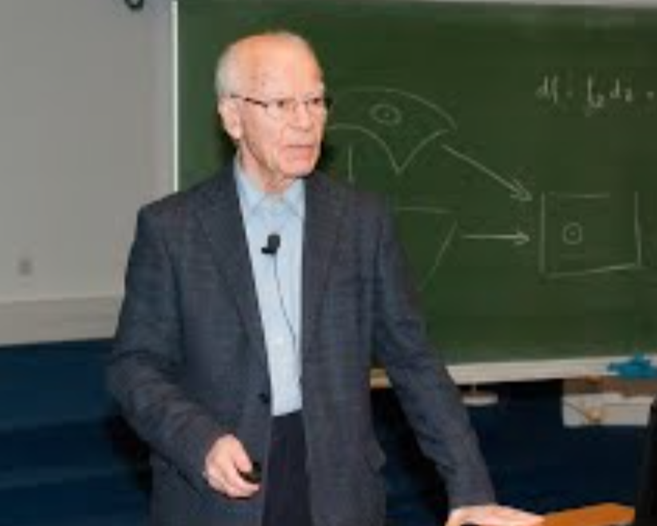
\includegraphics[width=0.7\textwidth]{Zorich.png}
\caption{В.А. Зорич во время лекции}
\label{fig:zorich}
\end{figure}

\newpage
\section{Список литературы}
\begin{thebibliography}{1}

\bibitem{zorich}
В.А.Зорич.
\textit{Математический анализ. Часть 1}.

\end{thebibliography}

\end{document}
